\chapter{Results}
In this chapter, we present the models created during the project.
We also present the criteria for choosing the best model, and we evaluate the model on the testing data.
Then we present the results.


\section{Pipeline}
During this project, we created a reproducible pipeline.
This pipeline can download the required data and preprocess them in a way that is suitable as an input to the neural networks models.
The pipeline is then able to create a model based on our specification and train it on the training dataset.

\section{Model comparison}
With the pipeline, we tested multiple models for classification problems.
These models were validated using our validation set.
We applied this method to two different problems - prediction of tissue type and prediction of cancer stage.

\subsection{Tissue type prediction}
The best models for tissue type of prediction were the models with parameters \verb'naive_ff_57992-26' and \verb'naive_ff_57992-100-26'.
These models were fully connected and used all the possible genes in the dataset.
In advance, the first model did not contain any hidden layer and therefore is equivalent to a simple linear transformation.
The second model uses one hidden layer with 100 hidden units and ReLU activation function.
The models achieved validation accuracy of 98.48\%
We noticed that the model with a hidden layer attained this level of accuracy sooner during the training, but also appeared to be more variable.

We also tried to decrease the number of units in the input layer.
This approach performed the best predictors selection since our genes were sorted according to the variance of the within-group means, and principal components were sorted by descending variance explained.
Unfortunately, no improvement of the model accuracy was achieved by this.

Another experiment, which we performed, was the use of the custom Pathways layer.
Despite the introduction of new information to the models, the models performed poorly in comparison with simple feedforward neural networks.

In total, we constructed and measured the performance of 12 models with different parameters.
The measured validation accuracy across the epochs is visualized in Figure \ref{fig:val_acc_tt}.

\begin{figure}
    \centering
    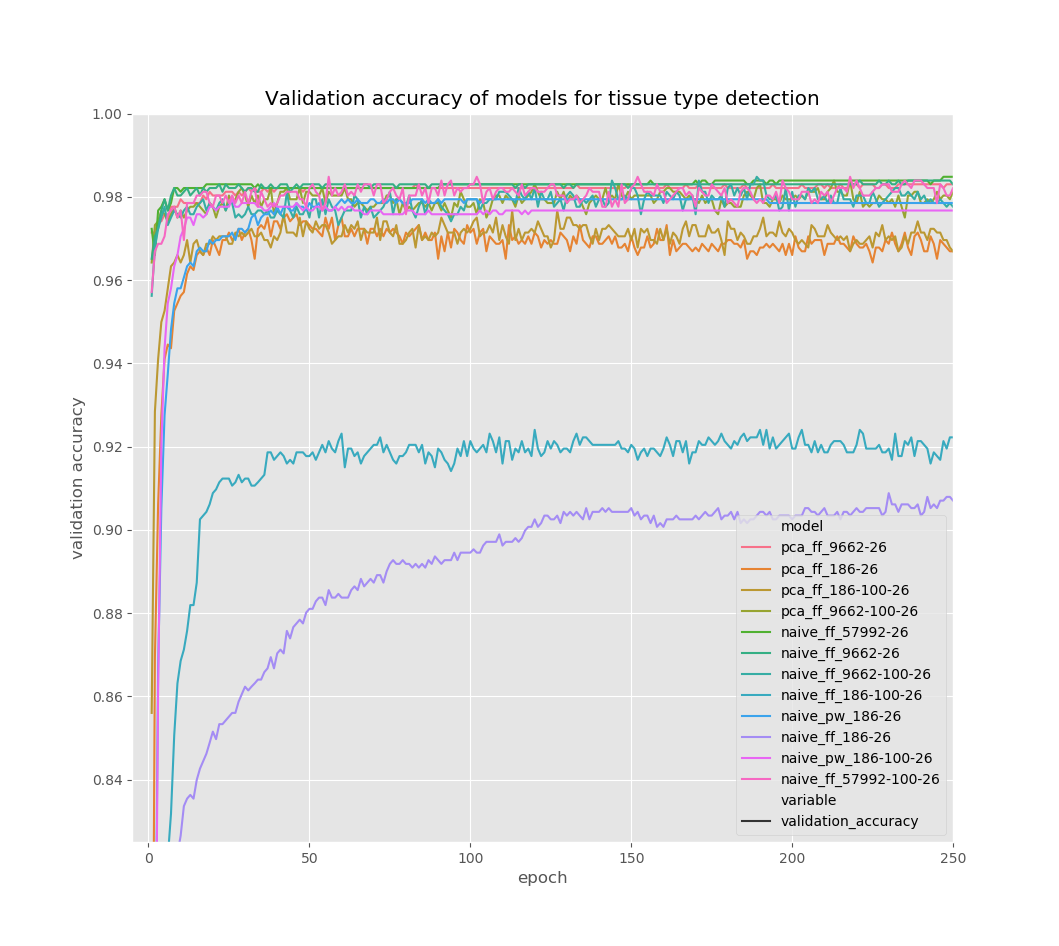
\includegraphics[width=\linewidth]{images/val_acc_tt_v2.png}
    \caption[Validation accuracy - tissue type]{Validation accuracy of tissue type prediction across the epochs using models with different architectures}
    \label{fig:val_acc_tt}
\end{figure}

\subsection{Prediction of cancer stage}
The best models for stage prediction were the models with parameters \verb'pca_ff_9662-100-5', \verb'naive_ff_9662-100-5' and \verb'naive_ff_57992-100-5'.
The first of these models used all principal components of a PCA transformed data.
The second of these models used 9662 genes with the highest variance of the within-group means.
The third of these models used all genes.
In all cases, the data were then run through one hidden layer with 100 hidden units and ReLU activation.
The resulting validation accuracy of the models was 52.5\%.
Even though this accuracy is very low in comparison with the accuracy in the previous problem, it is an improvement over the random model, which would yield accuracy around 20\%.

In this case, we performed similar experiments as in the case with tissue type prediction.
The reduction of the input size did not improve the accuracy, as all of the models with the maximal number of predictors performed equally.
We noticed that the model \verb'naive_ff_9662-100-5' made use of the reduction of the input size without the decrease in accuracy.

The Pathway layer experiment again showed decreased effectiveness of the model, but at least was comparable with some other architectures with low performance.

We also measured the validation accuracy of created models across the epochs and visualized it in Figure \ref{fig:val_acc_st}.

\begin{figure}
    \centering
    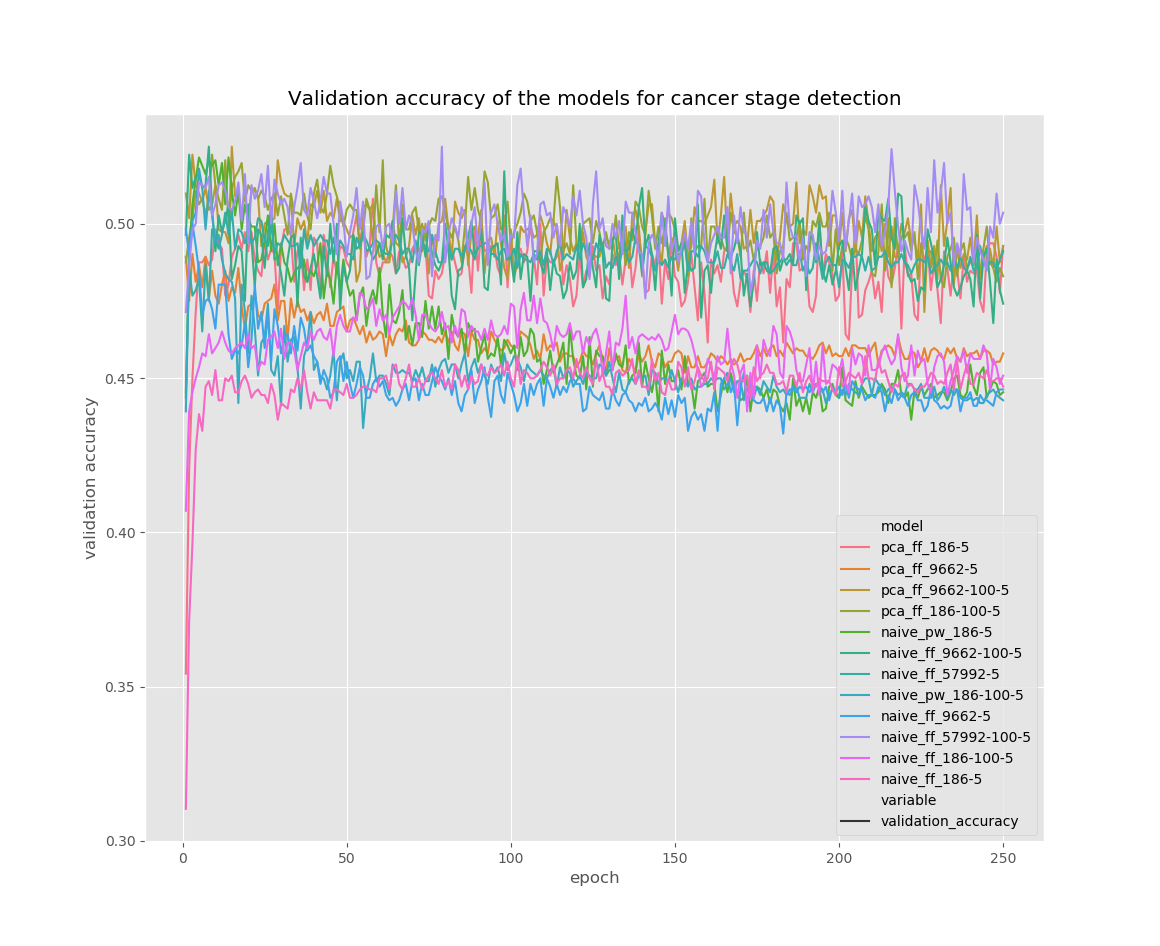
\includegraphics[width=\linewidth]{images/val_acc_st_v2.png}
    \caption[Validation accuracy - stage]{Validation accuracy of stage prediction across the epochs using models with different architecture}
    \label{fig:val_acc_st}
\end{figure}
